\documentclass{article}

\usepackage{graphicx}

\topmargin=-0.5cm
\leftmargin=-2cm
\rightmargin=0cm
\oddsidemargin=0cm
\evensidemargin=2cm
\textwidth=16.5cm
\textheight=20cm

\pagestyle{plain}

\begin{document}

\large

\vbox{}
\vspace{-2cm}
\begin{figure}[!ht]
%\hspace{-4mm}

\includegraphics[width=5cm]{img/logo.png}
\vspace{4mm}
\end{figure}
\noindent
\begin{center}
{\Huge Linear Elasticity Module}\\[2mm]
Based on Hermes2D ({\tt http://hpfem.org/hermes})\\[6mm]
\end{center}
\section{Module Description}

The linear elasticity module calculates displacements and stresses 
caused by deforming\footnote{Linear elasticity assumes that stress is a linear function of strain, and thus is applies to small deformations only.} solid objects. 
The objects can consist of one or more material subdomains with generally different values of the Young modulus $E$ and 
Poisson ratio $\nu$. In these subdomains, the material is assumed homogeneous.

\begin{figure}[!ht]
\begin{center}
%\hspace{-4mm}
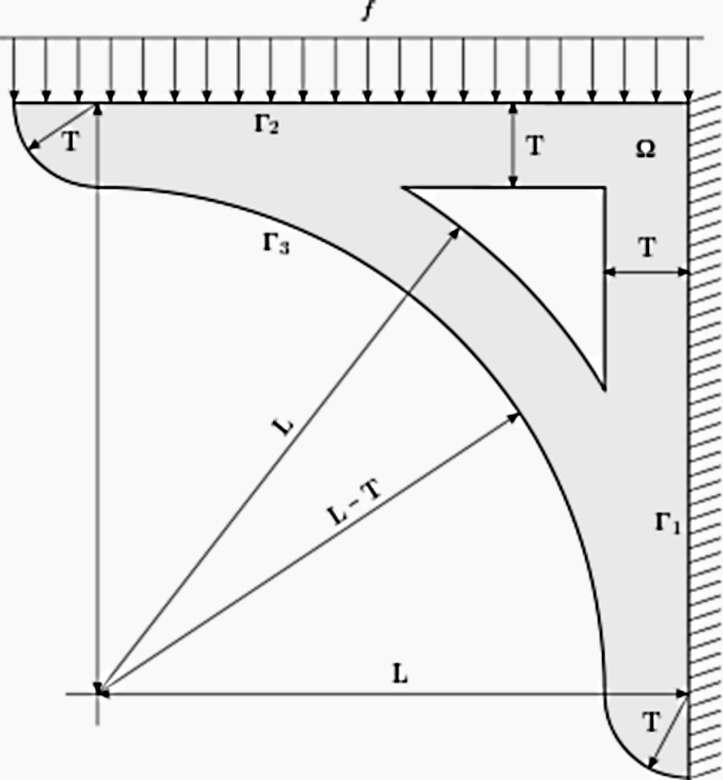
\includegraphics[width=8cm]{img/elastsample1.png}
\caption{Steel bookshelf bracket.}
\vspace{4mm}
\end{center}
\end{figure}
\noindent
On the boundary, one can prescribe {\em displacements} (right vertical edge 
in Fig. 1), {\em surface force} (top edge), or nothing (curved parts and the 
inner triangle). Prescribing nothing is equivalent to prescribing zero surface force. 
The model accounts for volumetric forces caused by the gravity or another acceleration. 
Calculated are displacements and the Von Mises stress.


\section{Underlying Equations}

Equations of linear elasticity consist of {\em equilibrium equations},
{\em strain-displacement equations} and {\em constitutive equations}.
Omitting their derivation (which can be found in many textbooks as well as 
on Wikipedia), the equations have the form 
$$
\mu u_{i, jj} + (\mu + \lambda) u_{j, ij} + F_i = 0, \ \ \ i = 1,2
$$
(Einstein's summation over repeated indices is used). 
Here $u_1, u_2$ are unknown displacements, $F = (F_1, F_2)$ the 
vector of volumetric forces, and $\lambda, \mu$ are Lam\'e constants.
If just gravitational acceleration is present, then we have 
$$
(F_1, F_2) = (0, -\varrho g)
$$
where $\varrho$ is the material density and $g$ the gravitational acceleration.
The Lam\'e constants $\lambda$
and $\mu$ are related to $E$ and $\nu$ as follows:

$$
\lambda = \frac{E \nu}{(1 + \nu)(1 - 2\nu)}, \ \ \ \mu = \frac{E}{2(1 + \nu)}.
$$

\section{Boundary Conditions}

There are two types of boundary conditions:
\begin{itemize}
\item {\em Fixed displacement}: $u_1 = u^*_1$ and $u_2 = u^*_2$ where $u^*_1, u^*_2$ are constants.
      Setting these constants to zero means a fixed boundary that does not move, but nonzero 
      boundary displacement can be also prescribed if deformation of the boundary is known. 
      It is possible to prescribe different displacements on different parts of 
      the boundary. 
\item {\em Surface force}: $f_1 = f^*_1$ and $f_2 = f^*_2$ where $f^*_1, f^*_2$ are constants.
      It is possible to prescribe different surface forces on different parts of 
      the boundary.
\item {\em Free boundary}: Where neither displacement nor surface force is prescribed, the
      boundary remains free. This is equivalent to prescribing $f_1 = 0$ N and $f_2 = 0$ N.
\end{itemize}

\section{Sample Results}

The following results correspond to the geometry from Fig. 1 with 
$E = 200$ GPa, $\nu = 0.3$, $\varrho = 8000$ kg/m$^3$,
$g = 9.81$ ms$^{-2}$, $F_1 = 0$ N, and $F_2 = -1000$ N.

\newpage
\begin{figure}[!ht]
\begin{center}
%\hspace{-4mm}
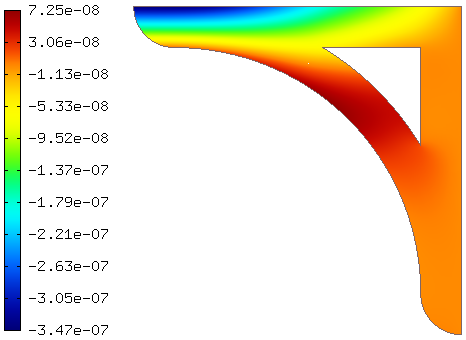
\includegraphics[width=7.5cm]{img/result-1.png}\ \ \ \ \ \ 
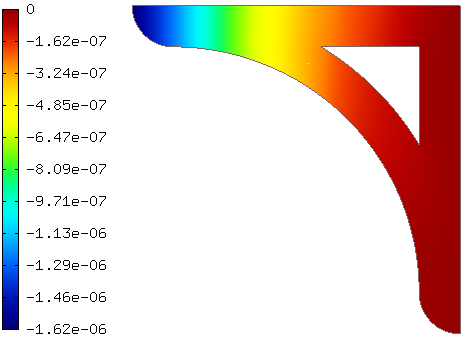
\includegraphics[width=7.5cm]{img/result-2.png}
\caption{Displacements $u_1$ and $u_2$.}
\vspace{4mm}
\end{center}
\end{figure}

\begin{figure}[!ht]
\begin{center}
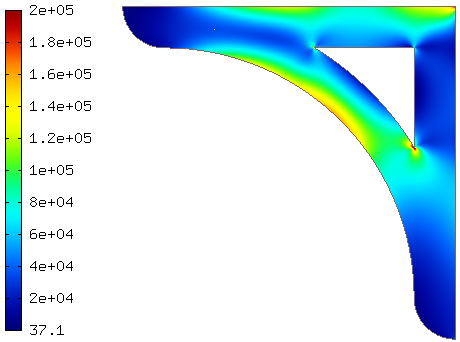
\includegraphics[width=7.5cm]{img/result-3.png}
\caption{Von Mises stress.}
\vspace{4mm}
\end{center}
\end{figure}
\noindent
In the last figure, notice singularities (pointwise infinite values) in the Von Mises 
stress at all three re-entrant corners. Singularities are a known difficulty of linear
elasticity models. They are easily underresolved if a coarse mesh is used. In order to 
resolve singularities accurately, adaptive finite element methods must be used. 
Adaptive $hp$-FEM methods that are provided by the Hermes library are among the 
best adaptive finite element methods available.

\end{document}

